\chapter{Clouds}\label{chp:LABEL_CHP_4}

One of the main applications of Ray Marching is in the rendering of realistic smoke, clouds, which are called volumetric objects. Clouds are mostly made of two main high-albedo types of particles, if not considering dirt or other minimal particles: air and water/ice \cite{:REF_IN_1}.
Since clouds are not solid, when light hits them, some rays bounce, but some go through the object. Not only that, the water particles are anisotropic \cite{:REF_IN_1}, which means that light tends to bounce differently depending on the direction from which it hits the cloud. All in all, there is a lot to adapt from the original Ray Marching. 

\section{Volumetric Rendering}

Firstly, to render gaseous materials, instead of avoiding going into surfaces, Ray Marching does need to traverse into them. For that, the SDF now represents density instead of ``distance to surface''. For the sake of clarity, the \texttt{GetDist(p)} will be renamed and modified so that it follows certain rules. This function is going to be called \texttt{GetDensity(p)}, and the rules are:

\begin{itemize}
    \item If \textbf{p} is \textbf{outside} of the primitive, yields a \textbf{negative} density, or no density.
    \item If \textbf{p} is \textbf{inside} of the primitive, yields a \textbf{positive} density, and the further \textbf{p} is from bounds, the higher density is.
\end{itemize}

Secondly, to consistently sample the density along the cloud, a constant step size is better suited. Instead of querying the scene's distance for the next marching step with the \texttt{GetDist} function, each iteration of the march step will have a constant size. Of course, this comes at the expense of performance, losing the optimizations discussed in Section 2.3.

To mitigate the loss, an outer bound will be applied to clouds. With a separate SDF, the bound will act as a regular surface, and when hit, Ray Marching will switch into the fixed step mode.

\begin{algorithm}[ht]
%\algsetup{linenosize=\tiny}
\caption{MarchRay}
\label{alg:marchray_cloud}
\begin{algorithmic}[1]
\Procedure{MarchRay}{Ray, Scene}
    \State $\mathbf{MarchDistance} \gets 0$
    \State $\mathbf{marchPos} \gets Ray.origin$
    \State $\mathbf{Hit} \gets \text{NULL\_HIT}$
    \State $\mathbf{accColor} \gets (0,0,0,0)$
    \For{$step \gets 0$ to $\text{MAX\_MARCH\_STEPS} - 1$}
        \State $\mathbf{marchPos} \gets Ray.origin + (MarchDistance \cdot Ray.direction)$
        \State $\mathbf{Hit} \gets \Call{GetDist}{marchPos, Scene}$
        \State $MarchDistance \gets MarchDistance + Hit.distance$
        
        \If{$Hit.distance < SURFACE\_DIST \ \land Hit.material \neq CLOUD$}
            \State $accColor \gets accColor + hitColor \cdot (1 - accColor.a)$
        \EndIf

        \If{$Hit.distance < SURFACE\_DIST \ \land \ Hit.material = CLOUD$}
            \For{$step \gets 0$ to $\text{FIXED\_MAX\_MARCH\_STEPS} - 1$}
                \State $MarchDistance \gets MarchDistance + \text{FIXED\_STEP\_SIZE}$
                \State $\mathbf{marchPos} \gets Ray.origin + (MarchDistance \cdot Ray.direction)$
                \State $\mathbf{Hit} \gets \Call{GetDist}{marchPos, Scene}$
                \State $\textbf{if } Hit.distance > 0 \ \land \ Hit.material \neq CLOUD \textbf{ then } \textbf{break}$
                \State $\mathbf{density} \gets \Call{GetDensity}{marchPos, Scene}$
                \If{$density > 0$}
                    \State $accColor \gets accColor + density \cdot (1 - accColor.a)$
                    \State $\textbf{if } accColor.a \geq 1 \textbf{ then } \textbf{break}$
                \EndIf
            \EndFor
        \EndIf

        \If{$MarchDistance > \text{MAX\_MARCH\_DIST} \ \lor \ accColor.a \geq 1$}
            \State \textbf{break}
        \EndIf
    \EndFor
    \State \Return $accColor$
\EndProcedure
\end{algorithmic}
\end{algorithm}

The pseudocode in Algorithm \ref{alg:marchray_cloud} builds upon Algorithm \ref{alg:marchray} to describe the relationship between clouds and regular surfaces. It's a lengthy, yet simple procedure in theory. The first difference comes with the addition of $\texttt{accColor}$, a 4D vector describing the RGBA channels. Red, blue and green fields store the accumulated color of the pixel and the alpha channel stores the accumulated density. This makes the variable $\texttt{isHit}$ deprecated. Since the $\texttt{accColor.a}$ channel ranges from 0 to 1, $\texttt{accColor.a = 1}$ means the ray path is now fully clouded, that being from a straight hard surface, or the accumulation of density between cloudy masses. Said check happens in lines 22 and 26.

Thanks to the use of outer bounds for the clouds, the optimized Sphere Tracing (Figure \ref{fig:spheretracing}) is kept as normal, up until a cloud bound is hit, at line 13. At this point, Fixed-Step Ray Marching begins, and either stops when a hard surface is hit (line 18) or when the vision is fully clouded (line 22). As discussed, the \texttt{GetDensity(p)} function outlined in Code 10 acts as the \texttt{GetDist(p)} for cloudy objects. An example of this cloudy sphere is shown in Figure \ref{fig:no-noise-cloud}. It certainly looks foggy, but still lacks the organic shapes of a conventional cloud.

\begin{lstlisting}[language=GLSL, caption={Code 10: Get density of spherical cloud}, label={lst:GetDensity}, float=ht]
float GetDensity(p){
    vec3 cloudCenter = vec3(0., 0., 0.);
    float cloudRadius = 2.0;
    return length(p - cloudCenter) - cloudRadius;
}    
\end{lstlisting}

\begin{figure}[ht]
    \centering
  
\includegraphics[width=.6\linewidth]{imagens/cloud-noise/no-noise-cloud.png}
  \captionof{figure}{Raymarched Sphere with density}
  \label{fig:no-noise-cloud}
\end{figure}

% @TODO: Inserir imagem da nuvem sem noise

\section{Shaping the Cloud with Noise}

The process of iteratively penetrating a surface to accumulate density data is already sufficient to render a transparent object. The gathered density is used as a transparent color and mixed with the background. However, clouds are not a homogeneous sphere. In fact, their appearance is quite noisy. To achieve a cloud-like appearance in our renders, it is necessary to break the uniformity of the sphere through randomness.

The core idea is to introduce some kind of variation into the \texttt{getDensity} function. However, directly adding a random value (a white noise), is insufficient for shaping the clouds. This approach would only result in a featureless foggy sphere with a noisy texture.

Instead, what is needed is a structured form of randomness, where nearby points in space produce similar values. This is the principle behind value noise: a grid of pseudo-random values is defined in space, and smooth interpolation is applied between them. The result is a texture that appears random but exhibits greater continuity due to the smoothing. A comparison of the white noise and value noise with their respective cloud renders is shown in Figure \ref{fig:cloud_noise}


% @TODO: Adicionar como o código de getDensity seria alterado

\begin{figure}[ht]
    \centering

    % Row 1
    \begin{minipage}{0.45\textwidth}
        \centering
        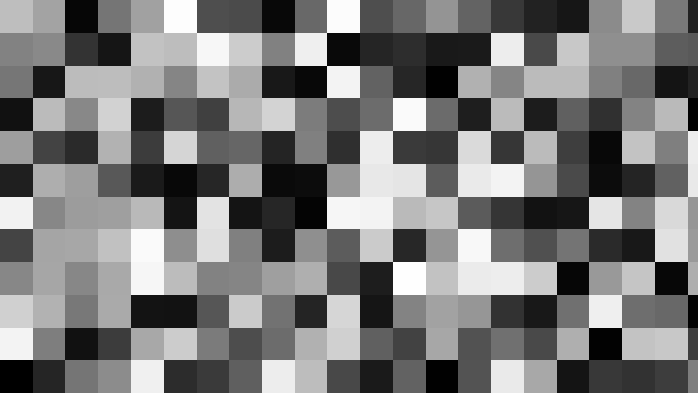
\includegraphics[width=\linewidth]{imagens/cloud-noise/white-noise.png}\\
        White Noise
    \end{minipage}%
    \hfill
    \begin{minipage}{0.45\textwidth}
        \centering
        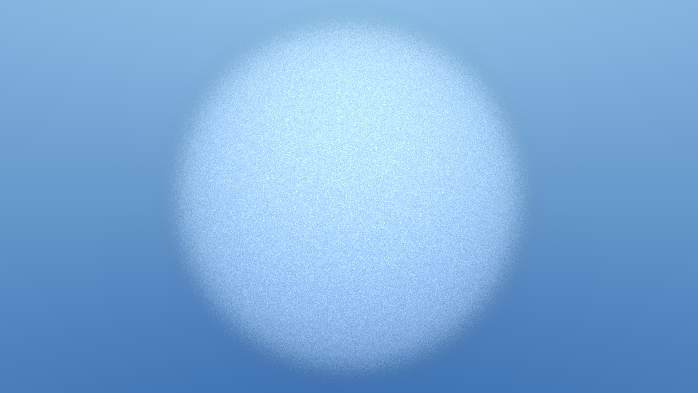
\includegraphics[width=\linewidth]{imagens/cloud-noise/white-noise-cloud.png}\\
        White Noise Cloud
    \end{minipage}

    \vspace{1em} % space between rows

    % Row 2
    \begin{minipage}{0.45\textwidth}
        \centering
        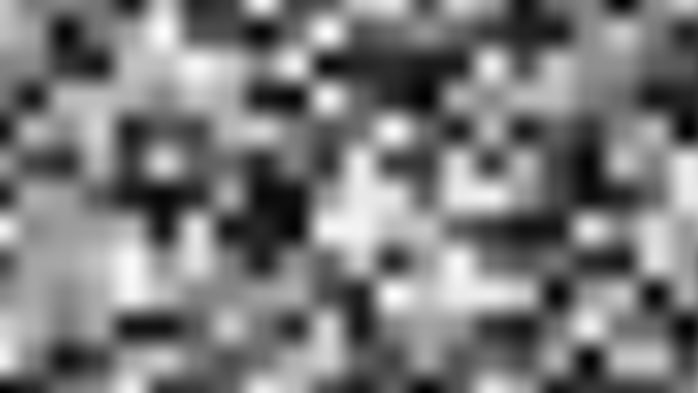
\includegraphics[width=\linewidth]{imagens/cloud-noise/value-noise.png}\\
        Value Noise
    \end{minipage}%
    \hfill
    \begin{minipage}{0.45\textwidth}
        \centering
        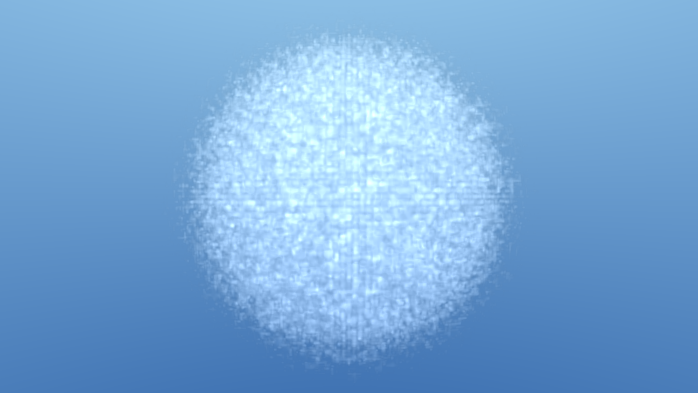
\includegraphics[width=\linewidth]{imagens/cloud-noise/value-noise-cloud.png}\\
        Value Noise Cloud
    \end{minipage}

    \caption{Comparison of White Noise and Value Noise for cloud generation.}
    \label{fig:cloud_noise}
\end{figure}

While value noise introduces a better variation, it still produces patterns that lack the complexity of a cloud. To overcome this limitation, multiple layers of noise can be combined at different scales in a technique known as fractal Brownian motion (fBm) \cite{MusgraveFractalTerrains}. For each iteration of the successive layer (or octave), a higher frequency and a lower amplitude are used. By applying fBm within the \texttt{getDensity} function, the cloud surface becomes more irregular and visually convincing, moving beyond a simple noisy sphere toward a shape that starts to resemble a cloud.

Figure \ref{fig:fbm_clouds} shows the 2D construction of the fBm, with each layer and the corresponding cloud render, where the noise is evaluated in three dimensions rather than two.

\begin{figure}[ht]
    \centering

    % Row 1: 1-Octave FBM Noise
    \begin{minipage}{0.45\textwidth}
        \centering
        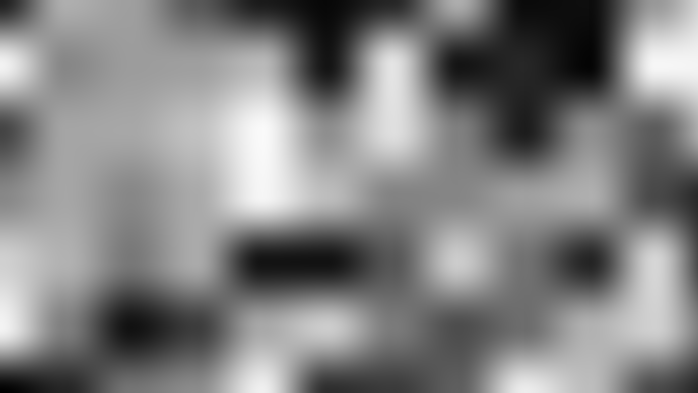
\includegraphics[width=\linewidth]{imagens/cloud-noise/1-octave-fbm.png}\\[0.3em]
        \small \texttt{valueNoise(uv)}
    \end{minipage}%
    \hfill
    % Row 1: 1-Octave Cloud
    \begin{minipage}{0.45\textwidth}
        \centering
        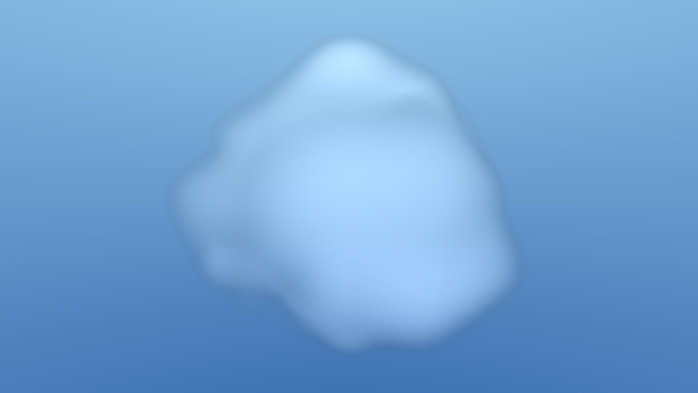
\includegraphics[width=\linewidth]{imagens/cloud-noise/1-octave-fbm-cloud.png}\\[0.3em]
        \small 1 Octave Cloud
    \end{minipage}

    \vspace{1em} % space between rows

    % Row 2: 2-Octaves FBM Noise
    \begin{minipage}{0.45\textwidth}
        \centering
        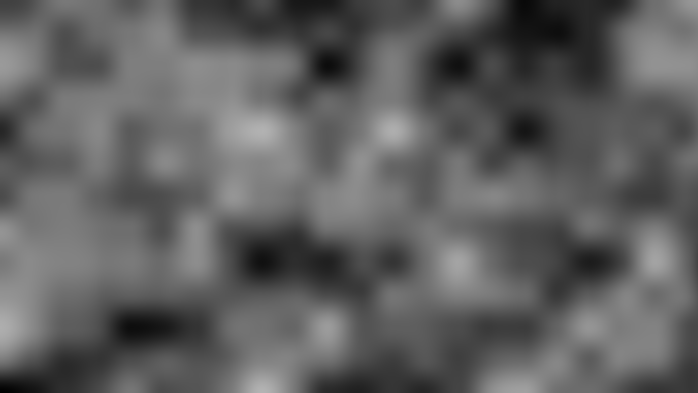
\includegraphics[width=\linewidth]{imagens/cloud-noise/2-octaves-fbm.png}\\[0.3em]
        \small \texttt{vn(uv)+vn(uv*2.)*0.5}
    \end{minipage}%
    \hfill
    % Row 2: 2-Octaves Cloud
    \begin{minipage}{0.45\textwidth}
        \centering
        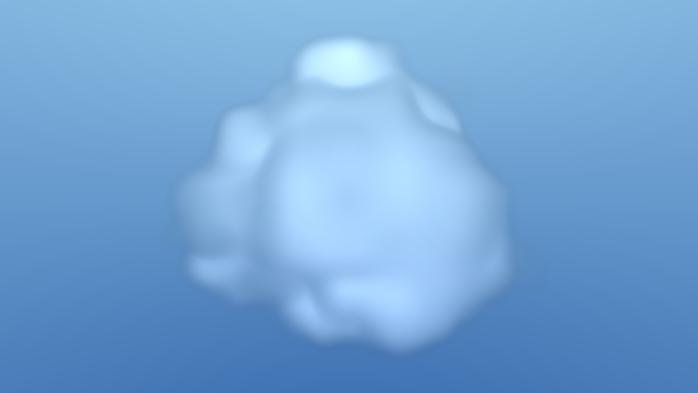
\includegraphics[width=\linewidth]{imagens/cloud-noise/2-octaves-fbm-cloud.png}\\[0.3em]
        \small 2 Octaves Cloud
    \end{minipage}

    \vspace{1em} % space between rows

    % Row 3: 3-Octaves FBM Noise
    \begin{minipage}{0.45\textwidth}
        \centering
        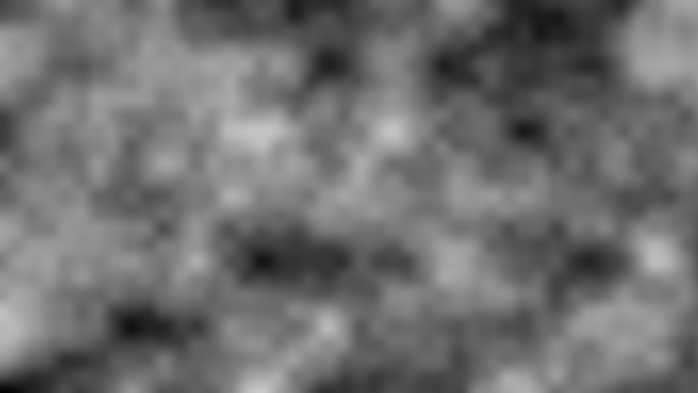
\includegraphics[width=\linewidth]{imagens/cloud-noise/3-octaves-fbm.png}\\[0.3em]
        \small \texttt{vn(uv)+vn(uv*2.)*0.5+vn(uv*4.)*0.25}
    \end{minipage}%
    \hfill
    % Row 3: 3-Octaves Cloud
    \begin{minipage}{0.45\textwidth}
        \centering
        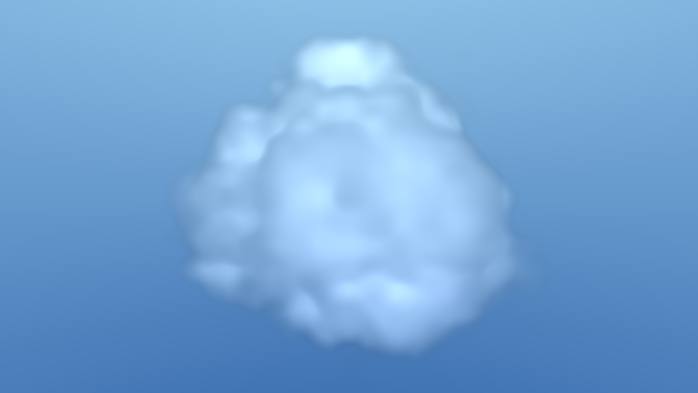
\includegraphics[width=\linewidth]{imagens/cloud-noise/3-octaves-fbm-cloud.png}\\[0.3em]
        \small 3 Octaves Cloud
    \end{minipage}

    \vspace{1em} % space between rows

    % Row 4: 4-Octaves FBM Noise
    \begin{minipage}{0.45\textwidth}
        \centering
        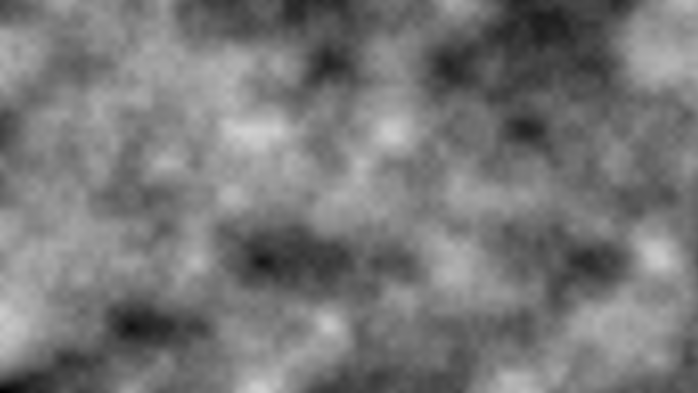
\includegraphics[width=\linewidth]{imagens/cloud-noise/4-octaves-fbm.png}\\[0.3em]
        \small \texttt{...vn(uv*4.)*0.25+vn(uv*8.)*0.125}
    \end{minipage}%
    \hfill
    % Row 4: 4-Octaves Cloud
    \begin{minipage}{0.45\textwidth}
        \centering
        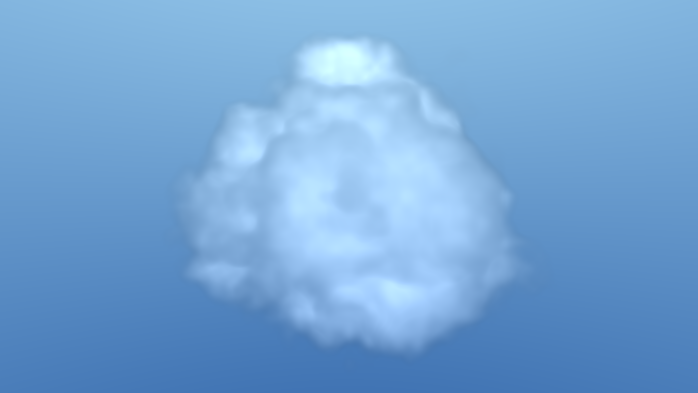
\includegraphics[width=\linewidth]{imagens/cloud-noise/4-octaves-fbm-cloud.png}\\[0.3em]
        \small 4 Octaves Cloud
    \end{minipage}

    \caption{FBM Noise and Corresponding Cloud Examples with Increasing Octaves.}
    \label{fig:fbm_clouds}
\end{figure}

\section{Volumetric Shading}

In the current implementation, cloud rendering does not account for the influence of 
scene illumination. To approximate the interaction between light and the volumetric 
medium, an efficient technique can be employed. At each sampling position, the algorithm 
advances a short distance along the direction of the incoming light and evaluates the 
density at this secondary location.  

At each sample location, we advance slightly along the light’s direction and measure the density again.

\begin{itemize}
  \item When the density is higher at the second position, the medium is locally thicker, resulting in increased light scattering
  \item When the density decreases, the cloud is less dense, leading to reduced scattering
\end{itemize}

This behaviour is illustrated in the implementation in Code 11.

\begin{lstlisting}[language=GLSL, caption={Code 11: Lighting the Cloud Volume}, label={CloudVolume} float=ht]
vec3 ldir = -normalize(light.direction);
vec3 li = light.color * (light.intensity / (4. * PI));
diffuse = clamp((getDensity(marchPos, scene) - getDensity(marchPos + 0.3 * ldir, scene)) / 0.3, 0.0, 1.0 );
accumulatedDiffuseColor += mix(vec3(0.), li, diffuse);
\end{lstlisting}

Because this technique only compares two nearby points, it is computationally inexpensive yet still captures the essential behavior of light within the volume.

It should be noted that this technique does not constitute a physically accurate 
simulation of light transport. In particular, it does not strictly follow Beer's law, 
which describes the exponential attenuation of light as it travels through a medium. 
Nevertheless, this approximation is sufficient for the purposes of our case study, as it is enough to produce visually convincing results in scenes with few light sources.

A demonstration of how this lighting approximation can produce compelling results is shown at Figure \ref{fig:lit-cloud}, displaying a raymarched cloud lit from a white directional light and a pink point light.

\begin{figure}[ht]
    \centering
    \fbox{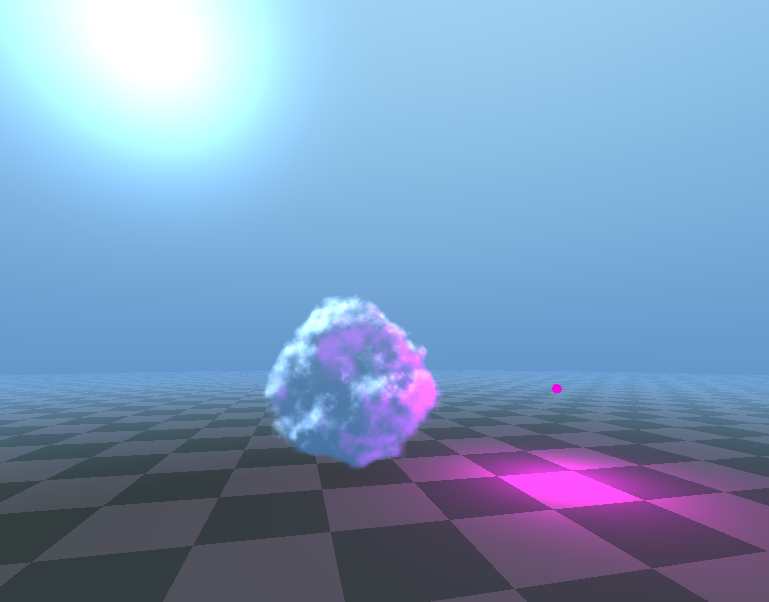
\includegraphics[width=9.5cm]{imagens/cloud-noise/lit-cloud.png}}
    \caption{Raymarched Cloud lit from directional light and point light}.
    \label{fig:lit-cloud}
\end{figure}

% Possível extra: Renderizar cena com SDFs diferentes de esfera para nuvem